\chapter{Je li Bog Osoba? - Članak John N. Loughborougha}

Jedan od najranijih članaka o \emcap{ličnosti Boga} je Loughboroughov članak “\textit{Je li Bog osoba?}” gdje on raspravlja o \emcap{ličnosti Boga} i Njegovoj prisutnosti. Važno je zapamtiti definiciju ‘ličnosti’ prema Merriam-Webster rječniku: “\textit{kvaliteta ili stanje koja nekog čine osobom}”\footnote{\href{https://www.merriam-webster.com/dictionary/personality}{Merriam-Webster Rječnik - ‘\textit{ličnost}’}}. Pažljivo ćemo pogledati kako Loughborough vidi kvalitetu ili stanje koja Boga čine osobom.

\begin{figure}[hp]
    \centering
    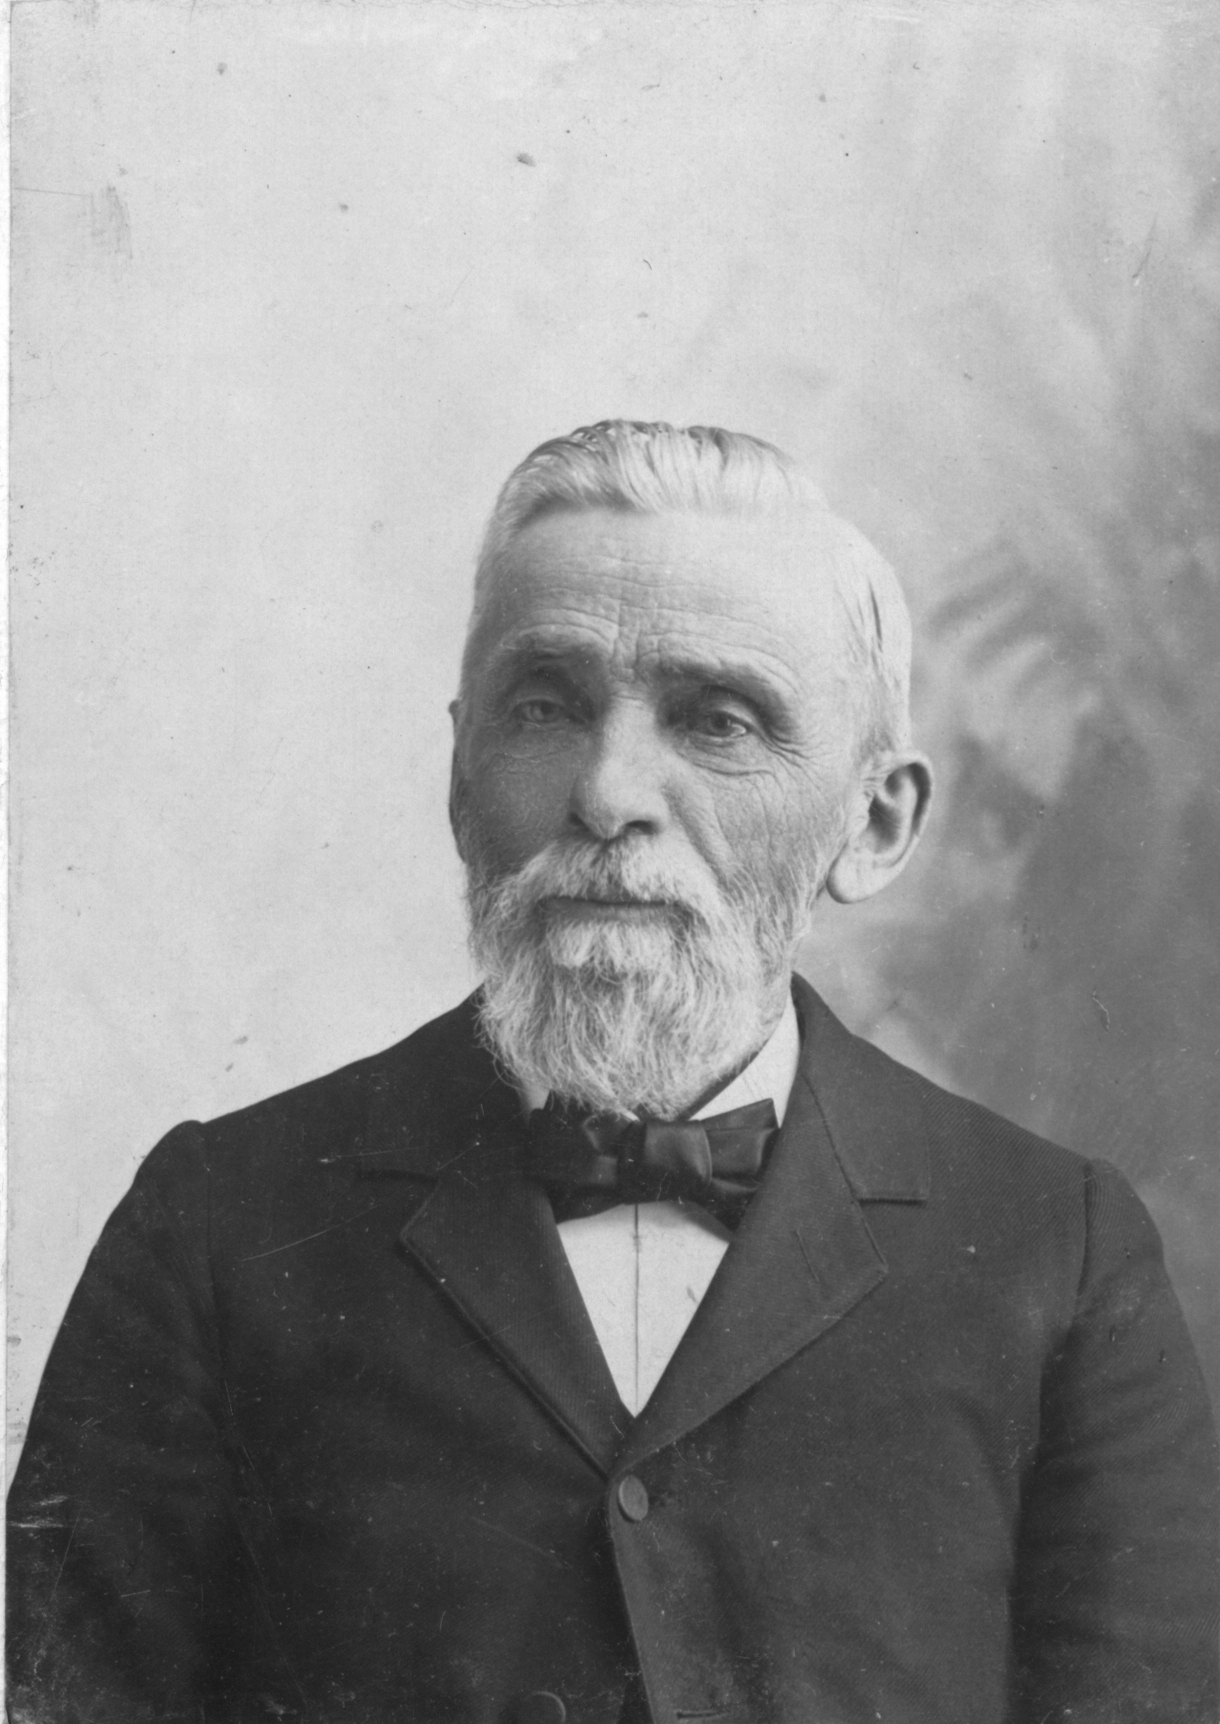
\includegraphics[width=1\linewidth]{images/john-n-loughborough.jpg}
    \caption*{John Norton Loughborough (1832-1924)}
    \label{fig:john-n-loughborough}
\end{figure}

\others{Što god bila istina po ovom pitanju, sigurno ne može biti pogrešno da istražimo što Riječ kaže o tome. \textbf{Mnogi se suzdržavaju od istraživanja nepopularnih istina jer se protiv njih diže optužba za herezu}. Ne smatramo se podložnima toj etiketi, \textbf{niti zadirujemo u tajne Svemogućeg dok nastavljamo s istraživanjem ove materije}. Biblija svakako sadrži svjedočanstva po ovom pitanju, i ponavljamo: ‘\textbf{Što je otkriveno, pripada nama}.’ Pitamo onda, što kaže Sveto pismo?}

\othersnogap{\textbf{Sâma svjedočanstva koja smo istraživali u vezi s činjenicom da je čovjek stvoren od praha zemaljskog na \underline{sliku Božju}, nedvosmisleno dokazuje da \underline{Bog ima oblik}, iako je to suprotno onome što smo učili kao djeca iz katekizma}:}

\othersnogap{Pitanje. Što je Bog?’}

\othersnogap{‘Odgovor. Beskonačni i vječni duh; onaj koji je uvijek bio i uvijek će biti.’}

\othersnogap{‘P. Gdje je Bog?’}

\othersnogap{‘O. Svugdje.’}

\othersnogap{\textbf{Ali pitamo, \underline{nije li Bog na jednom mjestu više nego na drugom}?} Oh ne, kažete vi: \textbf{Biblija kaže da je \underline{On duh}, i ako je tako, mora biti \underline{posvuda jednako prisutan}}. Po tome, znači, kada čovjek umre njegov duh ide Bogu, tada mora ići svugdje. \textbf{Ali Biblija svakako predstavlja Boga koji se nalazi na nebu. ‘Jer pogleda dolje sa svoje svete visine, GOSPOD s neba motri zemlju.’ Psalam 102:19}. \textbf{Onda svakako nebo ne može biti svugdje, jer se Bog prikazuje kako gleda odozgo. ‘\underline{Ilija uzađe} u vihoru \underline{na nebo}.’ 2. Kraljevima 2:11}. \textbf{Ali, kaže netko, zar Biblija ne prikazuje Boga kao \underline{sveprisutnog}?} Psalam 139:8, 9, 10. ‘Popnem li se na nebesa, \textbf{ti si ondje}; prostrijem li si postelju u Šeolu, \textbf{gle, ti si ondje}; uzmem li krila zorina pa se nastanim na kraju mora, \textbf{i ondje će me voditi ruka tvoja} i držat će me desnica tvoja.’}

\othersnogap{Mi odgovaramo, \textbf{odgovor je predstavljen u 7. retku, kako slijedi}: ‘\textbf{\underline{Kamo da odem od tvoga Duha}?} \textbf{i kamo da pobjegnem od \underline{tvoje prisutnosti}?}’ \textbf{Duh je \underline{Božji predstavnik}}. \textbf{Njegova sila se očituje gdje god On želi, kroz djelovanje Njegovog Duha}. Krist, kada je dao nalog učenicima, kaže: ‘Idite po svem svijetu i propovijedajte evanđelje svakom stvorenju, i evo! \textbf{ja sam s vama u sve dane do svršetka svijeta}.’ Sada, nitko ne bi tvrdio da je Krist bio osobno na zemlji otkako su učenici počeli ispunjavati ovaj nalog. \textbf{Ali njegov Duh je bio na zemlji; Tješitelj kojeg je obećao poslati.} \textbf{Tako se na isti način Bog očituje \underline{svojim Duhom} koji je također sila kroz koju On djeluje}. ‘A ako \textbf{Duh onoga} koji je uskrisio Isusa od mrtvih prebiva u vama, \textbf{onaj koji je uskrisio Krista} od mrtvih oživjet će i vaša smrtna tijela \textbf{\underline{po svome Duhu} koji prebiva u vama}.’ Rimljanima 8:11. \textbf{\underline{Ovdje je napravljena jasna razlika između Duha i Boga koji uskrisuje mrtve tim Duhom}}. \textbf{Ako je živi Bog Duh u najstrožem smislu te riječi, a istovremeno posjeduje Duha, onda odmah imamo neobičnu ideju o Duhu Duha, nešto što će trebati barem spiritualist da objasni}.}[The Adventist Review and Sabbath Herald, 18. rujna 1855][https://documents.adventistarchives.org/Periodicals/RH/RH18550918-V07-06.pdf]

Dopustite nam kratak komentar. Nadamo se da prepoznajete specifičnu temu o kojoj se ovdje raspravlja. Tema je prva točka \emcap{Fundamentalnih Principa} i tvrdnja da Bog ima oblik, jer je čovjek stvoren na Božju sliku. Takvo razumijevanje Božje ličnosti isključuje ideju da je Bog svugdje prisutan. Brat Loughborough je dao biblijske razloge za Božju sveprisutnost, zajedno sa sentimentom da je “\textit{Bog na jednom mjestu više nego na drugom}”. Bog je svugdje prisutan preko svog predstavnika, Svetog Duha, baš kao što je napisano u prvoj točki \emcap{Fundamentalnih Principa}. Dalje u ovoj raspravi, čitat ćemo da je Bog duhovno biće i posjeduje opipljivo, materijalno tijelo, za razliku od ideje da je On čisto duh.

\others{Postoji barem jedna nepremostiva teškoća na putu \textbf{onih koji vjeruju da je \underline{Bog nematerijalan}, i da nebo nije doslovno, \underline{locirano mjesto}: oni su prisiljeni priznati da je \underline{Isus tamo tjelesno, kao doslovna osoba}}; isti Isus koji je bio razapet, umro i pokopan, bio je uskrsnut iz mrtvih, \textbf{uzašao na nebo}, i sada je \textbf{s desne strane Boga}. \textbf{Isus je posjedovao tijelo i kosti nakon svojeg uskrsnuća}. Luka 24:39. ‘\textbf{Pogledajte moje ruke i moje noge, da sam to ja sam; opipajte me i vidite, }\textbf{\underline{jer duh nema tijela ni kostiju kao što vidite da ja imam}}.’ \textbf{Ako je Isus tamo na nebu s doslovnim tijelom od mesa i kostiju, možda je ipak nebo nakon svega doslovno mjesto, prebivalište za doslovnog Boga, doslovnog Spasitelja, doslovne anđele i uskrsnule besmrtne svete?} \textbf{\underline{Oh ne, kaže netko, ‘Bog je Duh.’}} Tako je Krist rekao ženi Samarijanki kod zdenca. \textbf{Ne slijedi nužno da zato što je Bog Duh, \underline{da nema tijelo}}. U Ivanu 3:6, Krist kaže Nikodemu, ‘\textbf{Što je rođeno od Duha, duh je}.’ \textbf{Ako je ono što je rođeno od Duha duh, onda po istom principu, ono što ima duhovnu narav je duh. Bog je \underline{duhovno biće}, njegova narav je duh, on nije smrtne naravi; \underline{ali to ne isključuje ideju da ima tijelo}}. David kaže, [Psalam 104:4,] ‘koji čini \textbf{svoje anđele duhovima};’ ipak \textbf{\underline{anđeli imaju tijela}}. Anđeli su se ukazali i Abrahamu i Lotu, i jeli su s njima. \textbf{Vidimo da ideja da su anđeli duhovi ne dokazuje da nisu doslovna bića}.}

\othersnogap{Zaključuje se, budući da Biblija kaže da je Bog Duh, da On nije osoba. Zaključak ne bi trebao biti temelj za argument. Velike biblijske istine su jasno navedene, i ne bi nam bilo dobro temeljiti doktrinu na zaključcima koji su \textbf{u suprotnosti s izričitim izjavama u Božjoj riječi}. Ako Pismo izričito \textbf{navodi da je Bog osoba, nije prikladno izvoditi zaključak iz teksta koji kaže ‘Bog je Duh,’ \underline{da On nema tijelo}}.}

\othersnogap{Sada ćemo predstaviti nekoliko tekstova \textbf{koji dokazuju da je Bog osoba}. Izlazak 33:18, 23. ‘I on (Mojsije) reče: Molim te, pokaži mi slavu svoju!’ Stih 20. ‘I reče: \textbf{Ne možeš vidjeti \underline{lice moje}, jer ne može čovjek vidjeti me i živjeti}.’ Stihovi 21-23. ‘I GOSPODIN reče: Evo, ima mjesto kod mene i ti ćeš stajati na stijeni. I dogodit će se, dok slava moja bude prolazila, da ću te staviti u pukotinu stijene i \textbf{zaklonit ću te \underline{rukom svojom} dok ne prođem}; i uklonit ću \textbf{ruku svoju}, i vidjet ćeš \textbf{\underline{leđa moja}}; ali \textbf{\underline{lice moje} neće se vidjeti}.’ \textbf{Ako je Bog \underline{nematerijalni Duh}, tada ga Mojsije nije mogao vidjeti; jer nam je rečeno da duh ne može biti viđen prirodnim očima}. \textbf{Tada ne bi bilo primjereno da Bog kaže da će staviti svoju ruku preko Mojsijeva lica dok prolazi (naizgled da ga spriječi da vidi Njegovo lice), jer ga ni nije mogao vidjeti}. \textbf{Niti možemo pojmiti kako bi nematerijalna ruka mogla spriječiti zrake svjetlosti da dođu do Mojsijevih očiju}. \textbf{Ali ako je tvrdnja istinita \underline{da je Bog nematerijalan}, i ne može biti viđen prirodnim okom, gornji tekst je potpuno suvišan}. \textbf{Kakvog smisla ima reći da je Bog stavio svoju ruku preko Mojsijeva lica, da ga spriječi od viđenja onoga što se ne može vidjeti}.}

\othersnogap{Kaže netko, vidim da ne možemo uskladiti stvar na drugi način, nego da je Mojsije vidio doslovno tijelo; ali to nije bilo Božje vlastito tijelo, \textbf{to je bilo tijelo koje je uzeo da bi se mogao pokazati Mojsiju}. \textbf{Mojsije nije mogao stvoriti ispravne predodžbe o Bogu osim ako On nije preuzeo neki oblik.} \textbf{Tako je Bog uzeo tijelo}. Ovo baca još goru sjenu na stvar nego prvi stav; \textbf{jer optužuje Boga za prijevaru; govoreći Mojsiju da će Ga vidjeti, dok prema ovom svjedočanstvu Mojsije zapravo nije vidio Boga, nego drugo tijelo}. Osoba mora sumnjati gotovo bez mogućnosti oporavka, koja bi pokušala tako mistificirati i poništiti snagu ovog svjedočanstva.}[Ibid.][https://documents.adventistarchives.org/Periodicals/RH/RH18550918-V07-06.pdf]

Prepoznajete li da se brat Loughborough bavi sentimentom koji će dr. Kellogg predstaviti u Živom Hramu 48 godina kasnije? Dr. Kellogg je rekao da je istina da se Bog predstavio u \others{\textbf{\underline{određenom obliku ili mjestu}}}[Dr. John H. Kellogg, The Living Temple, str. 31.][https://archive.org/details/J.H.Kellogg.TheLivingTemple1903/page/n31/] jer \others{mora postojati nešto \textbf{opipljivije}, više \textbf{\underline{ograničeno}}, na što se um može usredotočiti u bogoslužju}[bid, str. 30][https://archive.org/details/J.H.Kellogg.TheLivingTemple1903/page/n30/], ali da je On, u stvarnosti, \others{\textbf{daleko izvan našeg shvaćanja \underline{kao što su granice prostora i vremena}}}[Ibid, str. 33][https://archive.org/details/J.H.Kellogg.TheLivingTemple1903/page/n33/]. Brat Loughborough razumno se usprotivio ideji da se Bog samo manifestira čovjeku kao određeno Biće, ali u stvarnosti nije ono što se predstavlja da jest. Takva tvrdnja \others{optužuje Boga za prijevaru}. Brat Loughborough nastavlja s potvrdnim, biblijskim svjedočanstvom da je Bog materijalno biće.

\others{Izlazak 24:9. ‘Tada se popnu Mojsije i Aron, Nadab i Abihu, i sedamdeset starješina Izraelovih: \textbf{i vidješe Boga Izraelova}: i pod \textbf{njegovim nogama} bijaše kao pod od safira, i kao samo nebo po čistoći.’ Bilo im je dopušteno \textbf{vidjeti njegove noge}, ali nijedan \textbf{čovjek ne može vidjeti njegovo lice i živjeti}. \textbf{Nijedno \underline{smrtno oko} ne može podnijeti zasljepljujući sjaj te slave Božjeg lica}. Daleko nadmašuje sunčevu svjetlost. Jer prorok kaže: ‘Svjetlost mjesečeva bit će kao svjetlost sunčeva, a svjetlost će sunčeva biti \textbf{sedam puta jača}, kao svjetlost od sedam dana, u dan kad Gospodin zavije ranu svojega naroda i izliječi udarac njihove rane.’ Izaija 30:26. Unatoč toj sedmerostrukoj svjetlosti koja će tada sjati, prorok govoreći o tom prizoru kaže: ‘Tada će se mjesec zastidjeti i sunce posramiti, kad Gospodin nad vojskama zacaruje na gori Sionu i u Jeruzalemu, pred starješinama svojim u slavi.’ Izaija 24:23. Ivanovo svjedočanstvo je [Otkrivenje 21:23] ‘I grad ne treba ni sunca ni mjeseca da mu svijetle, jer \textbf{ga obasja slava Božja}, i njegovo je svjetlo Janje.’}

\othersnogap{\textbf{Nevjernici tvrde da postoji proturječnost u Mojsijevom svjedočanstvu, jer je rekao da je razgovarao s Bogom licem u lice}. \textbf{Odgovaramo, između njih je bio oblak}, ali Bog je rekao Mojsiju: ‘\textbf{Nijedan čovjek ne može me vidjeti i ostati živ}.’ Svjedočanstvo Novog zavjeta je u skladu s onim Starog zavjeta o ovom predmetu. ‘Težite za mirom sa svima i za posvećenjem, bez kojega \textbf{nitko neće vidjeti Gospodina}.’ Hebrejima 12:14. \textbf{Tko bi \underline{smrtnim očima} mogao gledati svjetlost koja sedam puta nadmašuje sjaj sunca?} Zasigurno nitko osim svetih ne može ga vidjeti, \textbf{samo besmrtne oči} mogu podnijeti tu blistavu slavu. Iako Riječ kaže da sada ne možemo vidjeti Boga i živjeti, obećanje je da će ga \textbf{čisti srcem vidjeti}. Matej 5:3. ‘Blago čistima srcem, \textbf{jer će Boga gledati}.’ Otkrivenje 22:4. ‘I \textbf{gledat će njegovo lice}, a njegovo će ime biti na njihovim čelima.’}

\othersnogap{Pavao [Kološanima 1:15] govoreći o Kristu, kaže: ‘On je slika \textbf{nevidljivoga Boga}, prvorođenac svakog stvorenja.’ Ovdje se za Krista kaže da je ‘\textbf{slika nevidljivoga Boga}.’ Već smo pokazali da \textbf{Krist ima tijelo sastavljeno od tvari, mesa i kostiju; i za njega se kaže da je} ‘\textbf{slika nevidljivoga Boga}.’ Pa dobro, kaže netko, priznajemo da je njegova božanska priroda na sliku Božju. Ako pod njegovom božanskom prirodom mislite na dio koji je postojao u slavi s Ocem prije postanka svijeta, odgovaramo, ono što je bilo u početku s Bogom (Riječ), \textbf{postalo je tijelo, nije ušlo u tijelo}, ili kako neki kažu, \textbf{zaodjenulo se ljudskom prirodom, nego postalo tijelo}. Ali kaže drugi, \textbf{za Boga se kaže da je nevidljiv}. \textbf{To što je sada nevidljiv, ne dokazuje da nikada neće biti viđen}. Riječ kaže: ‘Čisti srcem \textbf{vidjet će ga}’. Voljna vjera kaže, Amen.}

\othersnogap{Pavlovo svjedočanstvo u Filipljanima 2:5, 6, jasno pokazuje što se može razumjeti pod izjavom da je Krist slika Božja. ‘Neka u vama bude isto mišljenje kao i u Kristu Isusu: koji je \textbf{bio u obličju Božjem}, nije smatrao otimačinom \textbf{biti jednak Bogu}.’ \textbf{Kako se može reći da je Krist u obličju Božjem, ako Bog nema obličja?} Rimljanima 8:3. ‘Bog poslavši svoga vlastitog Sina u obličju grešnog tijela.’ \textbf{Krist je u obličju Božjem i u obličju ljudi. Ovo nam odmah otkriva obličje Božje}.}

\othersnogap{\textbf{\underline{Daniel govoreći o Bogu, naziva ga Pradavnim}}. Daniel 7:9. ‘I Pradavni sjede, \textbf{čija odjeća bijaše bijela kao snijeg}, i \textbf{kosa njegove glave} kao čista vuna.’ \textbf{Za ovu osobu se kaže da ima glavu i kosu; to se zasigurno ne bi moglo reći za njega} \textbf{\underline{kad bi bio nematerijalan i bez oblika}}. \textbf{Ali Pavlovo svjedočanstvo u \underline{Hebrejima 1:3}, trebalo bi riješiti svaku iskrenu sumnju u \underline{vezi ličnosti Boga}}. Govoreći o Kristu, on kaže: ‘Koji budući sjajnost slave njegove, \textbf{i savršena slika njegove (\underline{Očeve osobe})}.’ \textbf{Ovdje je jasno navedeno da \underline{Bog ima osobu}. Krist je savršena slika te osobe.} Tada možemo razumjeti Krista gdje kaže: ‘\textbf{Tko je vidio mene, vidio je Oca}.’ Ivan 14:19. \textbf{On nije mogao misliti da je on svoj vlastiti otac; jer kada se molio obraćao se svom Ocu kao drugoj osobi koja ga je poslala u svijet}. Nazivao se \textbf{Sinom Božjim}. \textbf{Stoga nije mogao biti Otac čiji je on bio sin}. Kada kaže: ‘Tko je vidio mene vidio je Oca,’ mora značiti da, kao što je \textbf{on bio savršena slika Očeve osobe, oni koji su vidjeli njega vidjeli su Očevu sličnost u njemu}.}[The Adventist Review and Sabbath Herald, 18. rujna 1855][https://documents.adventistarchives.org/Periodicals/RH/RH18550918-V07-06.pdf]

Važno je obratiti pažnju na biblijske dokaze koje brat Loughborough ističe u svjedočanstvu da Bog ima tijelo. Brat Loughborough pregledava nekoliko biblijskih odlomaka dokazujući da Bog ima materijalno tijelo, ali je nevidljivo našim smrtnim očima. Sestra White je napisala isto kada je rekla\egwinline{\textbf{Otac je sva punina Božanstva \underline{tjelesno}} i \textbf{nevidljiv je smrtnom pogledu}}. Nijedno smrtno oko ne može vidjeti Oca, ali to ne dokazuje da Bog nikada ne može biti viđen. Isus je rekao: \bible{\textbf{Tko je vidio mene, vidio je Oca}}[Ivan 14:19]. Isus je objasnio ove riječi dva poglavlja ranije: \bible{Isus povika i reče: Tko vjeruje u mene, ne vjeruje u mene, \textbf{nego u onoga koji me je poslao}. I \textbf{tko vidi mene vidi onoga koji me je poslao}}[Ivan 12:44-45]. Isus nije poslao samoga sebe, niti je Isus Otac, jedna te ista osoba; ali mi vidimo Oca u Kristu jer On je \textit{savršena slika Očeve osobe}. (Hebrejima 1:3). Kao što je Isus osoba, koja posjeduje tijelo, tako je i Otac. Brat Loughborough nastavlja dokazivati svoju poantu da je Bog osoba, koja posjeduje oblik i formu, jer je čovjek stvoren na Božju sliku.

\others{Ali sada ćemo se vratiti na temu stvaranja čovjeka. \textbf{Već smo vidjeli da to što je čovjek stvoren na sliku Božju, nije se moglo odnositi na moralnu sliku, jer bi to uključivalo apsurd da je beživotna glina od koje je čovjek oblikovan imala karakter poput Boga}. \textbf{Sada vidimo da Sveto pismo jasno uči da je \underline{Bog osoba s tijelom i oblikom}}. Tada se Postanak 1:26 može razumjeti da uči činjenicu \textbf{da je čovjek stvoren u obliku Božjem}. Drugi tekstovi se slažu s ovim svjedočanstvom. Vidi Postanak 9:6. ‘Tko prolije krv čovjekovu, njegovu će krv čovjek proliti: \textbf{jer na sliku Božju stvoren je čovjek}.’ \textbf{\underline{Ovo svjedočanstvo ne može se primijeniti na duh ili nematerijalni dio čovjeka: ono što je na sliku Božju ima krv}}. 1 Korinćanima 11:7. ‘Čovjek doista ne treba pokrivati glavu, \textbf{budući da je slika i slava Božja}.’ Jakov [Poglavlje 3:9] govoreći o jeziku kaže: ‘Njime blagoslivljamo Boga, Oca; i njime proklinjemo ljude \textbf{koji su stvoreni na sličnost (nalik, nalikovanje - Webster) Božju}.’ \textbf{Prethodno svjedočanstvo utvrđuje točku \underline{da se slika Božja ne odnosi na karakter nego na oblik}}.}

\othersnogap{Postanak 2:7. ‘\textbf{I Gospod Bog oblikova čovjeka od praha zemaljskoga i u nosnice mu udahnu dah života; i čovjek postade živa duša}.’}[The Adventist Review and Sabbath Herald, 18. rujna 1855.][https://documents.adventistarchives.org/Periodicals/RH/RH18550918-V07-06.pdf]

Bog je stvorio čovjeka na svoju sliku. Bog je osoba koja ima tijelo, oblik i formu, i On je stvorio čovjeka na svoju sliku. Iz ovog razmišljanja izvodimo očito značenje biblijskog svjedočanstva o \emcap{ličnosti Boga}. Ako stvorimo pogrešne koncepcije o Božjoj osobi, u opasnosti smo da pogrešno razumijemo druge istine koje su povezane s čovjekovom prirodom (smrtnost duše, stanje mrtvih, itd.). U svom članku, brat Loughborough nastavlja objašnjavati vezu između lažne doktrine o besmrtnosti duše i pogrešnih koncepcija o \emcap{ličnosti Boga}. Njegov članak u Review and Herald od 18. rujna, preuzet je iz njegove knjige “\textit{Ispitivanje Biblijskog Svjedočanstva}”\footnote{\href{https://egwwritings.org/?ref=en_MPC.2&para=961.2}{John Norton Loughborough, An Examination of the Scripture Testimony, 1855}}.

% Je li Bog osoba? - prema članku Johna N. Loughborougha

\begin{titledpoem}
    \stanza{
        Bog na prijestolju sjedi, kao osoba stvarna, \\
        Ne kao duh bez oblika, što je zabluda davna. \\
        Duhovno tijelo ima, iako našim očima skriveno, \\
        Previše sjajno za smrtnike, Pismom otkriveno.
    }

    \stanza{    
        Sveprisutan je Bog kroz Duha svog, \\
        Kao predstavnika moći, Lika tog. \\
        "Tko je vidio mene, vidio je Oca" - Krist zbori, \\
        Jer savršenu sliku Očeve osobe On tvori.
    }

    \stanza{
        Na Božju sliku stvoreni smo mi, \\
        U obliku, ne samo u naravi. \\
        Osoba prava s tijelom stvarnim jest, \\
        Ne magla bezoblična, kako neki žele svest.
    }

    \stanza{
        Bog jeste svepristuan, ali ne svugdje jednako, \\
        Na Nebu tijelom, a svugdje Duhom samo tako.
        Jednog dana čisti srcem će Ga vidjeti, \\
        Pred nogama Njegovim, će Ga obožavati.
    }
\end{titledpoem}